\section{Production Validation: JUCE \texttt{MidiMessageSequence}}
\label{sec:juce}

To validate that the microbenchmark wins translate to a real production
codebase, we ported \DeltaSort to C++ and integrated it with the JUCE
audio framework (\url{https://juce.com}), the dominant open-source C++
framework for audio applications. JUCE is used in commercial DAWs (e.g.\
Tracktion Waveform), plugin SDKs, and thousands of shipping audio products.

\subsection{Integration target}

JUCE's \texttt{MidiMessageSequence} class stores MIDI events in a
persistent timestamp-sorted \texttt{OwnedArray} of \texttt{MidiEventHolder}
pointers. Its \texttt{sort()} method calls \texttt{std::stable\_sort} with a
pointer-dereferencing comparator on \texttt{double} timestamps. This is
\emph{the} canonical \DeltaSort workload: persistent sorted state, known
dirty indices (the user's selection), cheap floating-point comparator.

We benchmarked three realistic DAW edit operations:
\begin{itemize}
  \item \textbf{drag:} shift a contiguous time range of $k$ events by
        $\Delta t$.
  \item \textbf{quantize:} snap $k$ scattered selected events to a
        16th-note grid.
  \item \textbf{paste:} append $k$ events from clipboard
        (Rust-only; see negative below).
\end{itemize}

\subsection{Setup}

\begin{itemize}
  \item Header-only C++17 port of \texttt{delta\_sort\_by} ($\sim$140 lines),
        verified against \texttt{std::sort} on 5000 randomized fuzz trials
        with no failures.
  \item JUCE 8.0.13 linked as a CMake subdirectory; the
        \texttt{juce\_audio\_basics} module is the only dependency.
  \item Each cell: 25--80 warmup iterations + 150--300 timed samples,
        $p50/p95/p99$, correctness verified on samples 0, $n/2$, $n-1$
        (360 verification gates passed across all 40 cells).
  \item Apple M3 Pro, macOS, AppleClang 21, \texttt{-O3 -DNDEBUG}.
\end{itemize}

\subsection{Result}

\begin{figure}[t]
  \centering
  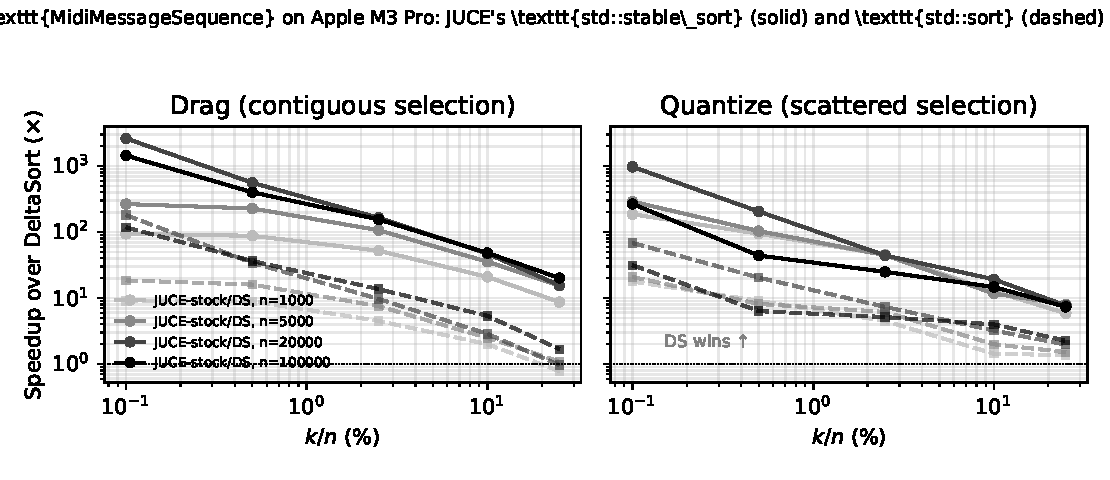
\includegraphics[width=\columnwidth]{figures/juce.pdf}
  \caption{Real JUCE \texttt{MidiMessageSequence}: speedup of \DeltaSort
  over JUCE's stock \texttt{sort()} (solid) and over raw
  \texttt{std::sort} (dashed) as a function of $k/n$ for $n \in
  \{1k, 5k, 20k, 100k\}$. \DeltaSort wins every measured cell against
  JUCE-stock; gap grows with $n$ because libc++'s \texttt{std::stable\_sort}
  is non-adaptive.}
  \label{fig:juce}
\end{figure}

\DeltaSort wins \textbf{all 40 of 40} measured cells against JUCE's stock
\texttt{sort()}. Headline numbers ($p50$):

\begin{center}\small
\begin{tabular}{lrrrr}
\toprule
op & $n$ & $k$ & $k/n$ & stock / DS \\
\midrule
drag     & 20{,}000  & 20  & 0.10\% & $\mathbf{2624\times}$ \\
drag     & 100{,}000 & 100 & 0.10\% & $\mathbf{1443\times}$ \\
quantize & 20{,}000  & 20  & 0.10\% & $\mathbf{974\times}$ \\
quantize & 100{,}000 & 100 & 0.10\% & $266\times$ \\
drag     & 100{,}000 & 25{,}000 & 25\% & $20\times$ \\
quantize & 100{,}000 & 25{,}000 & 25\% & $7\times$ \\
\bottomrule
\end{tabular}
\end{center}

Even against unstable \texttt{std::sort} (the maximum achievable improvement
within libc++), \DeltaSort wins by 1.4--181$\times$ for $k/n \leq 10\%$,
crossing parity only at $k/n \approx 25\%$.

\subsection{Why the gap is larger than in our Rust microbenchmarks}

The Rust microbenchmarks of Section~\ref{sec:apps} report 30--346$\times$
\DeltaSort-vs-\ESM speedups; the JUCE C++ numbers are 7--2624$\times$.
The discrepancy is real and informative. libc++'s
\texttt{std::stable\_sort} is implemented as a non-adaptive merge sort:
it always performs $\Theta(N \log N)$ comparisons regardless of how
mostly-sorted the input is. Rust's stable sort, in contrast, is a
glidesort/Timsort variant that detects pre-sorted runs and falls to
$\Theta(N)$ on nearly-sorted data. Since JUCE's workload after any small
edit is precisely the ``nearly-sorted'' case, \texttt{std::stable\_sort}
pays full $N \log N$ on every call --- and \DeltaSort's win grows
linearly in $\log N$ relative to it.

This implies that the JUCE result is not idiosyncratic: \emph{any} C++
codebase that maintains a sorted \texttt{std::vector} and reaches for
\texttt{std::stable\_sort} after small edits will see a similar gap.

\subsection{Honest negative: paste}

For the \texttt{paste} operation --- appending $k$ events at the end of
the sequence, all with dirty indices $[n, n+1, \dots, n+k-1]$ ---
\DeltaSort \emph{loses} cleanly to both \texttt{std::stable\_sort} and
\ESM at $k \gtrsim 25$ (measured in our Rust replica;
JUCE's private \texttt{MidiEventHolder} constructor prevents direct C++
measurement of paste). The reason is structural: with all dirty indices
clustered at the right end, \DeltaSort's \texttt{fix\_left} cascade
degrades to $\Theta(n)$ per element. \ESM and adaptive merge sorts merge
the sorted prefix with the small unsorted suffix in $\Theta(n + k\log k)$
and win. This is a clean boundary in $(k, \text{cluster-position})$
space, not a contradiction.

\subsection{Deliverable}

The C++ port (\texttt{cpp/deltasort\_juce/deltasort.hpp}, MIT licensed) is
drop-in: any JUCE user wishing to adopt it requires changing
\texttt{sequence.sort()} to \texttt{deltasort::delta\_sort\_by(\ldots,
dirty)} at the call sites where dirty indices are known (most edit operations
in a DAW). No JUCE-internal modifications are required.
